\documentclass[a4paper,11pt]{article}

%PAQUETES

\usepackage[left=2.5cm,top=2.5cm,right=2.5cm,bottom=2.5cm]{geometry}
\usepackage[pdftex]{graphicx}	% paquete para imagenes
\usepackage{latexsym,amsmath,amssymb,amsfonts,cancel}
\usepackage[activeacute,spanish]{babel} 	% paquete para tildes
\usepackage[utf8]{inputenc}		% paquete para español
\usepackage{multirow}	% paquete para poder poner texto multifila
\usepackage{multicol}	% paquete para poder poner texto multicolumna
%\usepackage{pdflscape}	% paquete para poder poner paginas horizontales
%\usepackage{rotating}	% paquete para rotaciones

\usepackage{hyperref}	% paquete para hiperenlaces
\hypersetup{
	bookmarks=false,
	pdfborder={0 0 0},
	colorlinks=true,
	linkcolor=black,
	citecolor=black,
	urlcolor=blue
}

%\usepackage{csvtools}	% paquete para cargar datos desde fichero csv
%\usepackage{csvsort}	% paquete para ordenar tablas csv

\usepackage{color, colortbl}
\definecolor{light-gray}{gray}{0.95}
\definecolor{myred}{RGB}{252,74,58}
\definecolor{mygreen}{RGB}{111,255,79}

\usepackage{listingsutf8}
% CARACTERISTICAS DE LOS ARCHIVOS DE CODIGO FUENTE
\lstset{
	language=Matlab,
	basicstyle=\small,
	keywordstyle=\color[rgb]{0.5,0,0}\bfseries,
	stringstyle=\color{blue},
	commentstyle=\color[rgb]{0,0.5,0},
	showstringspaces=false,
	numbers=left,
	numberstyle=\tiny,
	%stepnumber=5,
	numbersep=5pt,
	backgroundcolor=\color{light-gray},
	showspaces=false,
	showtabs=false,
	frame=single,
	framexleftmargin=10mm,
	frame=trBL,
	rulesepcolor=\color{black},
	tabsize=2,
	captionpos=b,
	breaklines=true,
	breakatwhitespace=false,
	inputencoding=utf8,
	extendedchars=\true
}

\DeclareGraphicsExtensions{.bpm,.png,.pdf,.jpg}	% extensiones de imagenes

% RENOMBRAMIENTO DE COMANDOS

\renewcommand{\figurename}{Figura}
\renewcommand{\tablename}{Tabla}

% para poner las secciones centradas con el comando 'ssection'
\newcommand{\ssection}[1]{%
  \section[#1]{\centering\normalfont\scshape #1}}

\newcommand{\sen}{\mathtop{\rm sen}\nolimits}
\newcommand{\arcsen}{\mathtop{\rm arcsen}\nolimits}
\newcommand{\arcsec}{\mathtop{\rm arcsec}\nolimits}

\def\max{\mathtop{\mbox{\rm mx}}}
\def\min{\mathtop{\mbox{\rm mn}}}

%\def\changemargin#1#2{\list{}{\rightmargin#2\leftmargin#1}\item[]}
%\let\endchangemargin=\endlist{}

% para personalizar el formato de los numeros de las secciones y subsecciones
\def\thesection{\Roman{section}} % poner numeros romanos en section
\def\thesubsection{\Alph{subsection}} % poner letras en subsection

%Para personalizar el formato de los titulos
\usepackage{pstcol}
\makeatletter
\def\LigneVerticale{\vrule height 4cm depth 2cm\hspace{0.1cm}\relax}
\def\LignesVerticales{%
  \let\LV\LigneVerticale\LV\LV\LV\LV\LV\LV\LV\LV\LV\LV}
\def\GrosCarreAvecUnChiffre#1{%
  \rlap{\vrule height 0.8cm width 1cm depth 0.2cm}%
  \rlap{\hbox to 1cm{\hss\mbox{\white #1}\hss}}%
  \vrule height 0pt width 1cm depth 0pt}
\def\@makechapterhead#1{\hbox{%
    \huge 
    \LignesVerticales
    \hspace{-0.5cm}%
    \GrosCarreAvecUnChiffre{\thechapter}
    \hspace{0.2cm}\hbox{#1}%
}\par\vskip 2cm}
\def\@makeschapterhead#1{\hbox{%
    \huge 
    \LignesVerticales
    \hspace{0.5cm}
    \hbox{#1}%
}\par\vskip 2cm}

%Para conseguir que en las páginas en blanco no ponga cabeceras
\makeatletter
\def\clearpage{%
  \ifvmode
    \ifnum \@dbltopnum =\m@ne
      \ifdim \pagetotal <\topskip
        \hbox{}
      \fi
    \fi
  \fi
  \newpage
  \thispagestyle{empty}
  \write\m@ne{}
  \vbox{}
  \penalty -\@Mi
}
\makeatother


\begin{document}

	%NUMEROS DE PAGINA NORMAL
	\renewcommand{\thepage}{\arabic{page}}
	\setcounter{page}{1}
	
	\begin{center}
	
		%TITULO
		\textbf{\LARGE{Teleoperation of a robotic arm made with Lego Mindstorm using an accelerometer sensor HiTechnic}}
		\vspace{0.5cm}
		
		%AUTOR - CENTRO
		Pérula Martínez, Raúl \flqq raul.perula@alumnos.uc3m.es \frqq\\
		Teleoperation and Telepresence in Robotic\\
		Carlos III University of Madrid
	
	\end{center}
	
	%CONTENIDO
	\begin{multicols}{2}

		\textbf{\textit{Abstract} -- Teleoperation in robotics is one of the most important topics today because there are not still autonomous systems with intelligence so great as to be very precise in the work that have to play. Therefore, research is much in this field to allow operators to have a precise robot management and in the easiest way possible. In the case developed, I has made the programming of a Lego Mindstorm robot formed by the shape of a robotic arm that can move in the same way that the operator moves.}\\

		\textbf{\textit{Index term} -- Lego Mindstorm, robotic arm, teleoperating control, accelerometer sensor.}
		
		\ssection{Introduction}

			From the beginning, robotics has looking for getting robots to perform a task the same way as human beings to. This is not easy to get, and sometimes impossible with the means that exist today. Thus, for tasks where there is great difficulty to perform, which requires a large enough precision or when intelligence needs to be high when there is any danger to do the task, usually makes use of the teleoperation.\\

			Teleoperation of the robot can be very useful in many cases because it is a practical way for a robot perform a task, either supervised or controlled by an operator. These tasks may be similar movements made by the operator withut any intermediate logic, or tasks in which the operator give instructions and the robot performs the action through a logic.\\

			In this work I have done a robotic arm made from Lego Mindstorms NXT system. Although it is not very complex system, you can see the features of teleoperation have and the utility it can offer to perform tasks more difficult in more complex systems.\\

			The following sections will study the key points to be treated by a teleoperated system and show in detail the programming and the structure of the robot.
		
		\ssection{Teleoperation system elements}
		
			This section describe what are the elements that the teleoperated system has, being this system a manipulator guided by an operator operator for several sensor and actuator elements.
			
			\begin{center}
				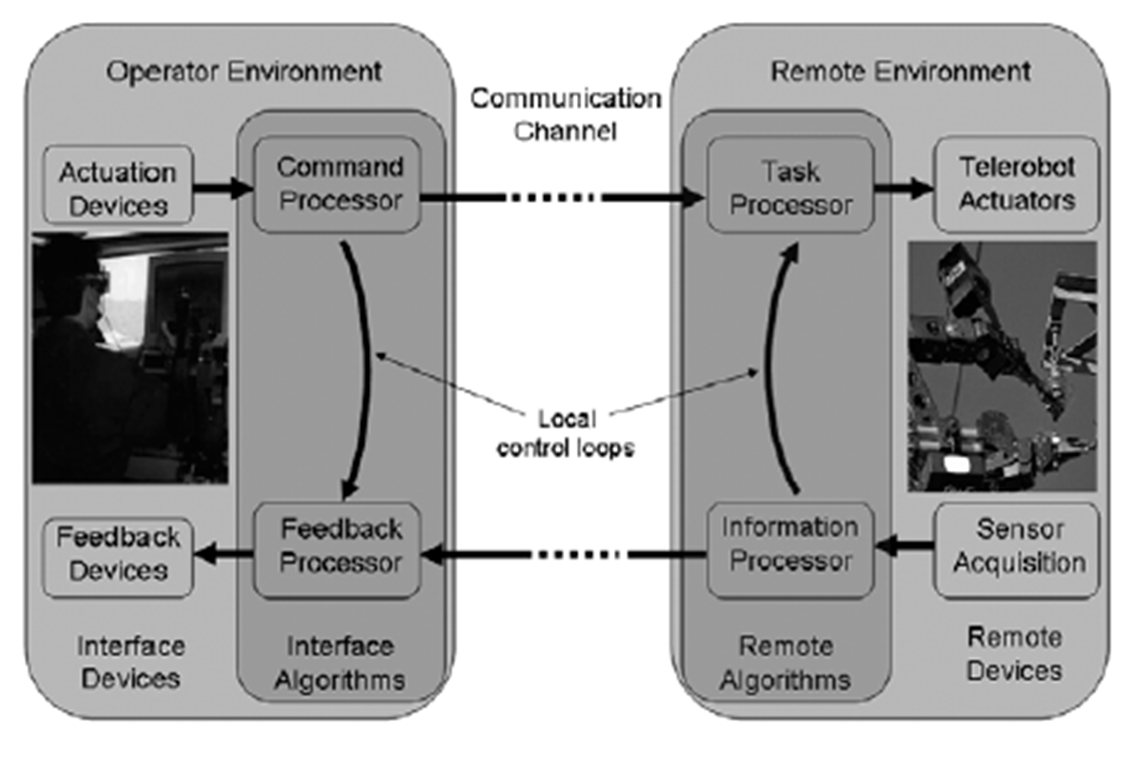
\includegraphics[scale=0.2]{img/environment.png}
				Environment teleoperated.
			\end{center}

			\subsection{Operator}

				The operator is the person responsible for managing or controlling the robot remotely. He will handle by hand controller (joystick) which shall consist on a couple of sensors that move the device.

			\subsection{Teleoperated device}

				The teleoperated device is the device in the remote area which is constrolled by the operator, this will be the robotic arm. It will consist of a mechanism in which the movement will be equal to that made by the operator. The robotic arm has two degrees of freedom to move around the three coordinate axes (3D). In the end, the robotic device will have a gripper to manipulate objects.
			
			\subsection{Sensors}

				One of the most important components of any robotic system are the sensors. These is a device that measures a physical quantity and converts it into a signal which can be read by an observer or by an instrument.\\
	
				The sensors used for this project have been:

				\begin{itemize}
					\item Acceleration sensor
					\item Touch sensor
				\end{itemize}

				Below are the characteristics of the sensors to have a little more information about it.\\

				\textbf{Acceleration sensor characteristics}\\

				NXT Acceleration Sensor contains a 3-axis accelerometer that measures the acceleration in 3 axes, X, Y and Z. The acceleration is measured in the range of -2g to +2 g with a resolution of approximately 200 units per g.\\

				\begin{center}
					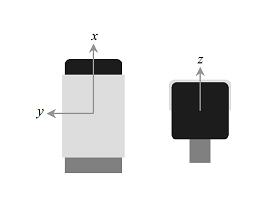
\includegraphics[scale=0.8]{img/sensorA.jpg}
					Acceleration Sensor
				\end{center}

				The acceleration sensor can also be used to measure the tilt in all 3 axes.\\
				
				The acceleration sensor connects to an NXT sensor port using a NXT standart cable via I2C digital communications protocol. The measurement of acceleration of each axis is updated 100 times per second.\\
				
				This sensor has been encapsulated in a similar way to other MINDSTORMS\textsuperscript{\textregistered} elements to maintain a coherent presentation.\\

				The value shown on the NXT represents the acceleration or inclination value for the X axis and will be in a range between 0 and 254.\\
				
				\textbf{Touch sensor characteristics}\\

				The NXT touch sensor consists of a piece that makes contact when it is pressed and sends a signal to recognize a keystroke.\\

				\begin{center}
					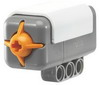
\includegraphics[scale=0.8]{img/sensorB.jpg}\\
					Touch Sensor
				\end{center}

				As shown in the figure, the sensor may have two positions, normal, in which there is no touch and we can say it is the resting position. And down position, which may be continuous or only one pulse.\\

				The value shown on the NXT represents if exist or not pulsation.

			\subsection{Interface}
			
				The interface to control the robotic device is provided by Lego Mindstorm. Based on block-structured programming that gives easy access to a variety of sensors and actuators that can operate the system. This way you can program the system how to behave in response to movements of the operator.
			
			\subsection{Control and communication channels}
			
				The control and communication channels are a collection of devices that modulate, transmit and adapt a set of signals which are transmitted between the local and the remote area. For this system, the communication channels are made using a data transmission cable standard NXT working via I2C digital communications protocol.
			
		\ssection{Teleoperation architecture}
		
			The architecture followed to implement the project has been a control supervised architecture.\\

			The figure shows the overall architecture is based on a system like this.\\
			
			\begin{center}
				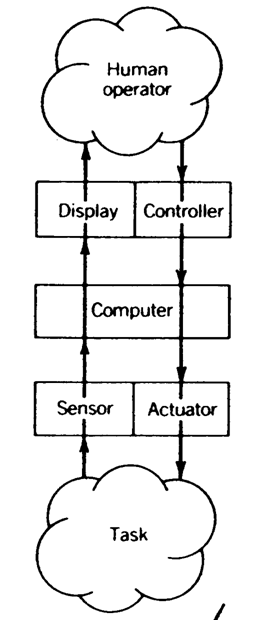
\includegraphics[scale=0.5]{img/architecture.png}\\
				Supervised control. Manual control architecture.
			\end{center}

			In our case, the operator is the person responsible for teleoperate the device as discussed above.\\

			The display to be used is the human eye, which can directly observe the movements of the device.\\

			The controller is the joystick that has been created which contains the acceleration sensor to capture the positions and directions that will have to replicate the device.\\

			\begin{center}
				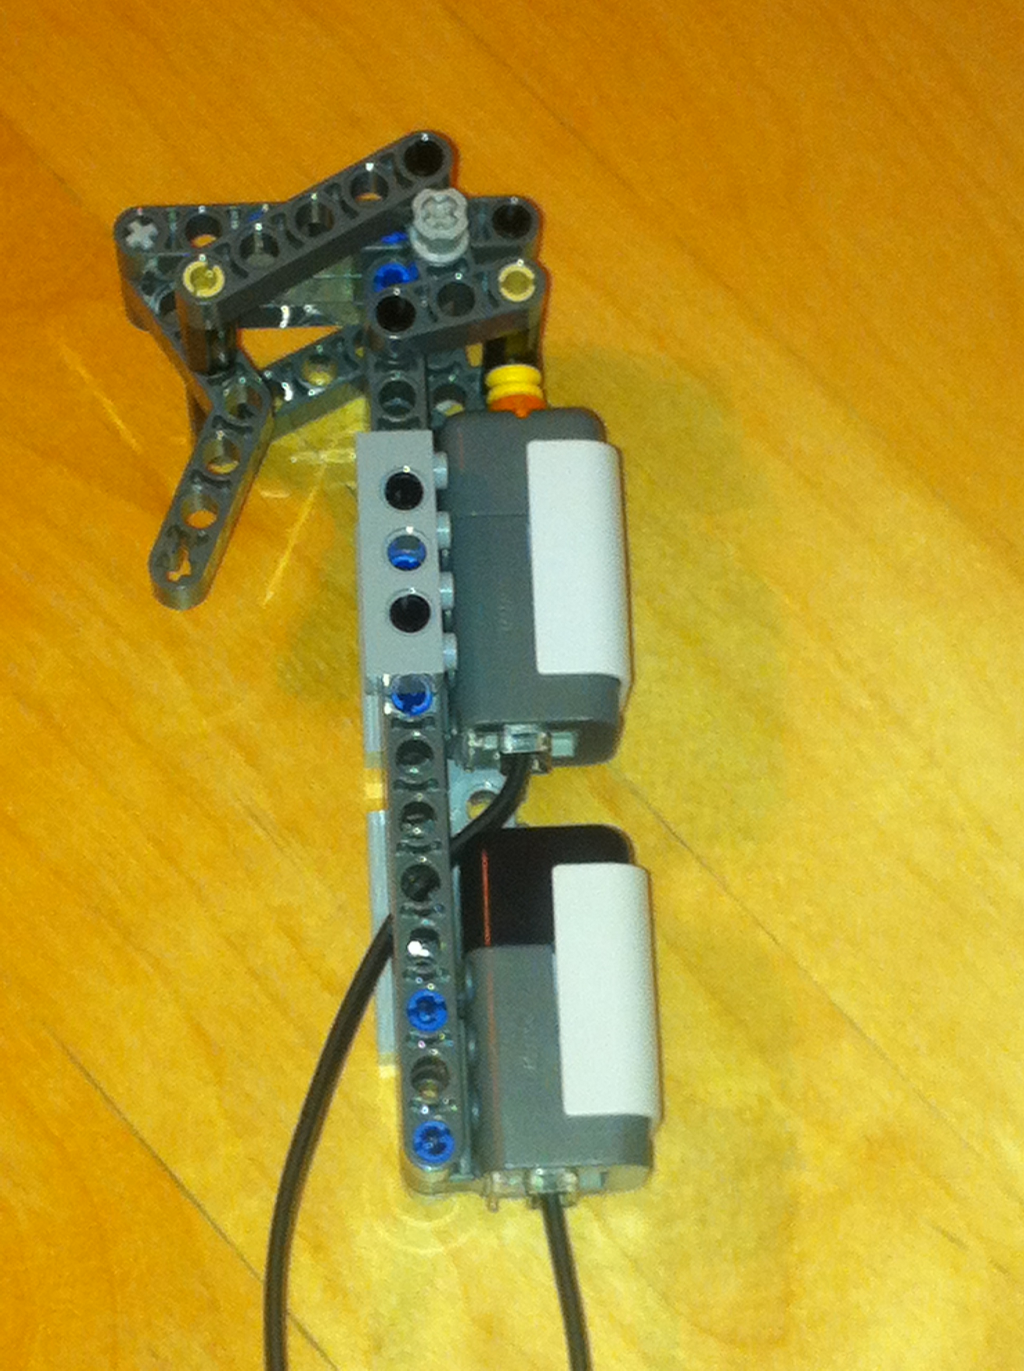
\includegraphics[scale=0.1]{img/joystick_left.png}\\
				Left perfil, joystick (sensors).
			\end{center}

			\begin{center}
				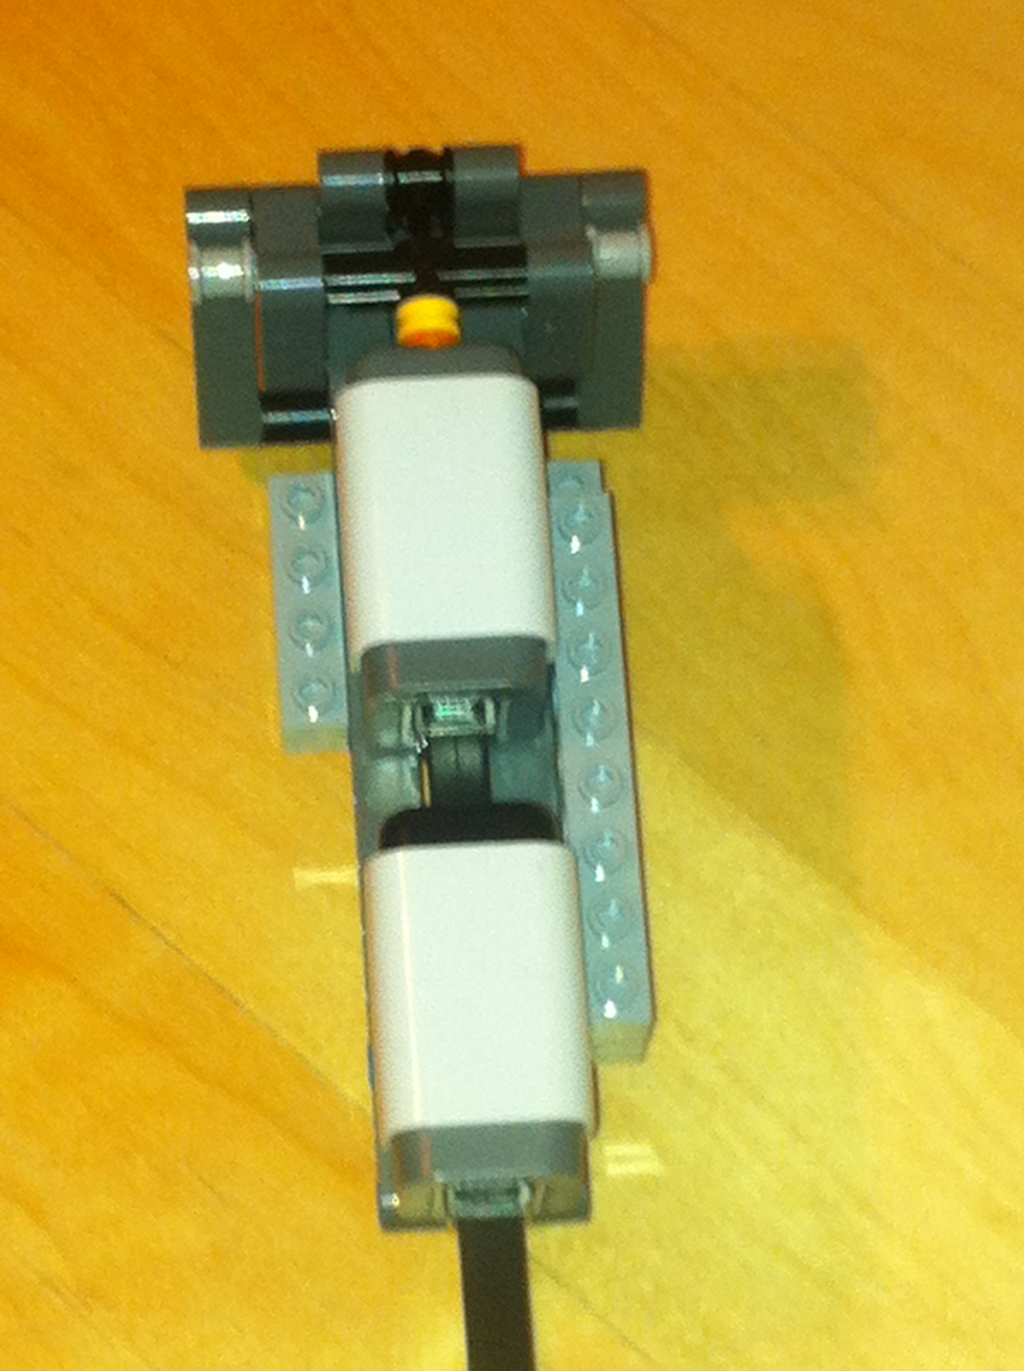
\includegraphics[scale=0.1]{img/joystick_front.png}\\
				Frontal perfil, joystick (sensors).
			\end{center}

			\begin{center}
				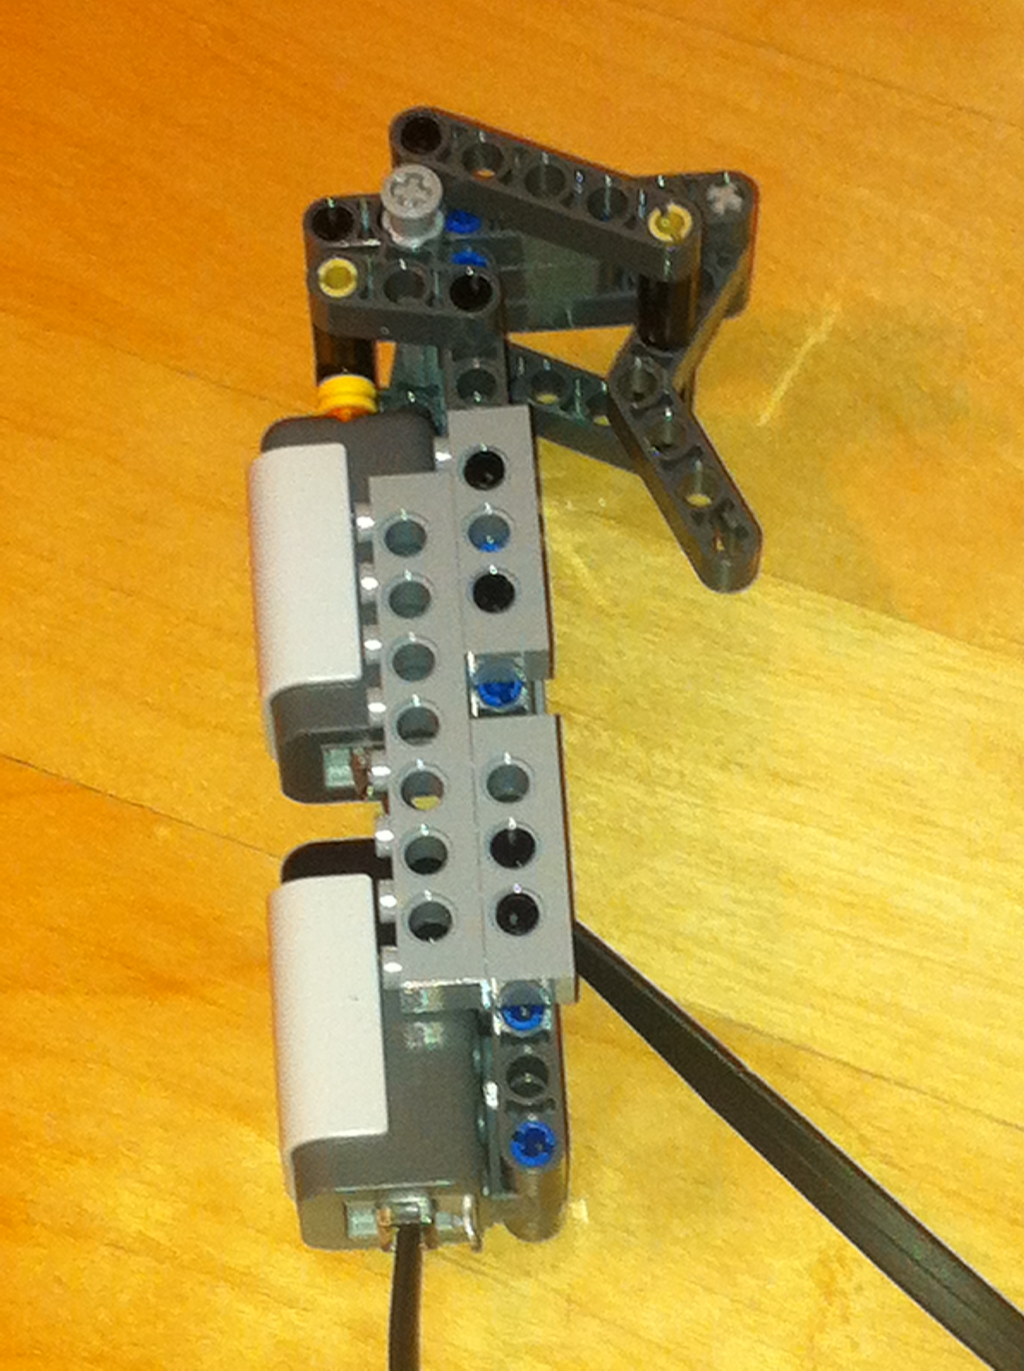
\includegraphics[scale=0.1]{img/joystick_right.png}\\
				Right perfil, joystick (sensors).
			\end{center}

			Sensors capture data necessary to perform their functions the actuators, causing the movement of the device and tasks are executed correctly.\\

			\begin{center}
				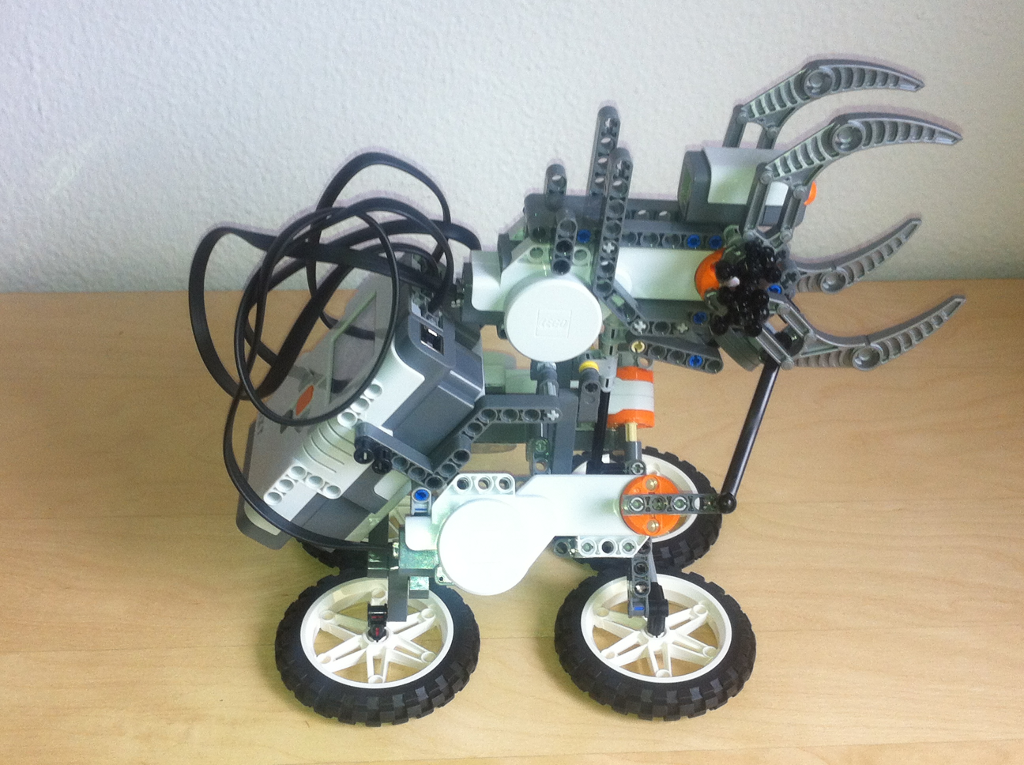
\includegraphics[scale=0.2]{img/robot1.png}\\
				Robotic device right (actuators).
			\end{center}

			\begin{center}
				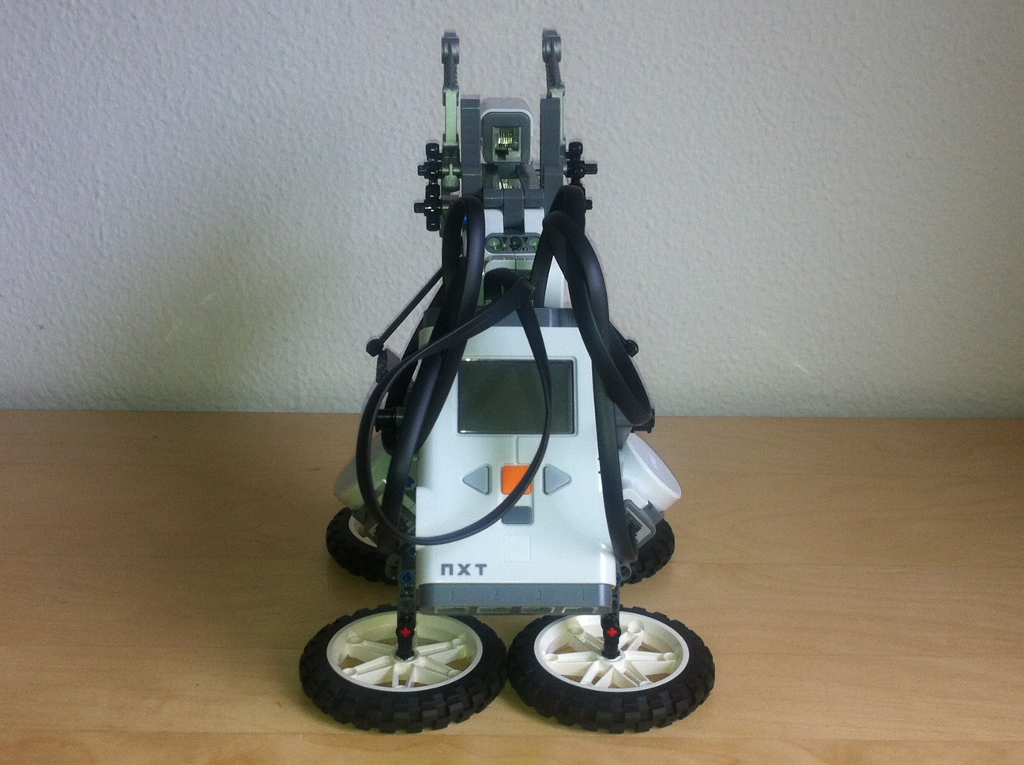
\includegraphics[scale=0.2]{img/robot2.png}\\
				Robotic device back (actuators).
			\end{center}

			\begin{center}
				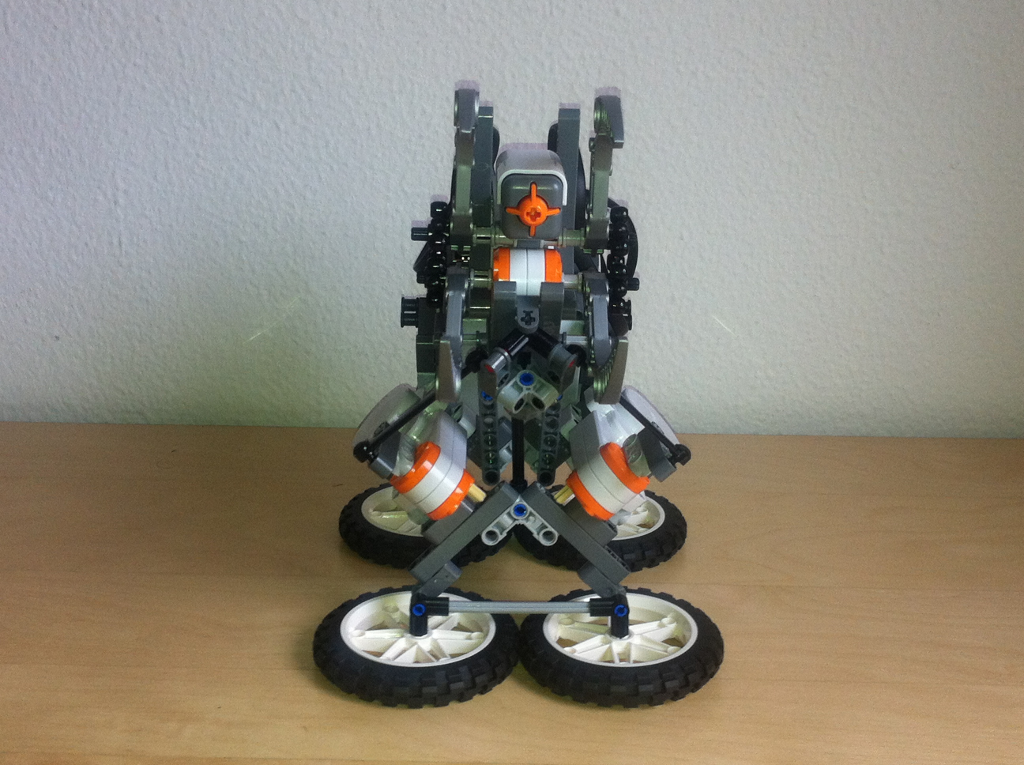
\includegraphics[scale=0.2]{img/robot3.png}\\
				Robotic device front (actuators).
			\end{center}

		\ssection{Control mode}

			In the master-slave control methodology, the slave robot (teleoperator) exactly replicates the movements of the master. Methods for controlling master-slave robot systems may be divided into two categories - unilateral control system and a bilateral control system. In a unilateral control system, shown in the figure, no force feedback is available from the slave unit. The only form of feedback to the master unit operator is in the form of vision data. Such a system has the merit of having a simple controller and mechanism; however dexterous manipulation is difficult.

			\begin{center}
				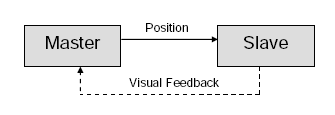
\includegraphics[scale=0.7]{img/master-slave.png}\\
				Unilateral master-slave control.
			\end{center}

			Most people find incredibly easy to use their arms as they have had so much practice. This natural ability of most human beings can be exploited to give a human operator an easy to use tool to control a robot.\\

			This system allows the user to move his hand in a natural way and the robot moves in the same way. In this manner the user is able to effectively and precisely manipulate the robot with very little training [3].

		\ssection{Software system}

			This section will explain the program which has been created to control and manipulate the robotic device, revealing each one of the blocks used.\\

			The figure shows the structure of the main program, you can observe two distinct parts. The first is responsible for performing control for the arm to move in the same way in which the operator moves the handle. And the second part controls the grip to catch things.\\

	\end{multicols}
	
			\begin{center}
				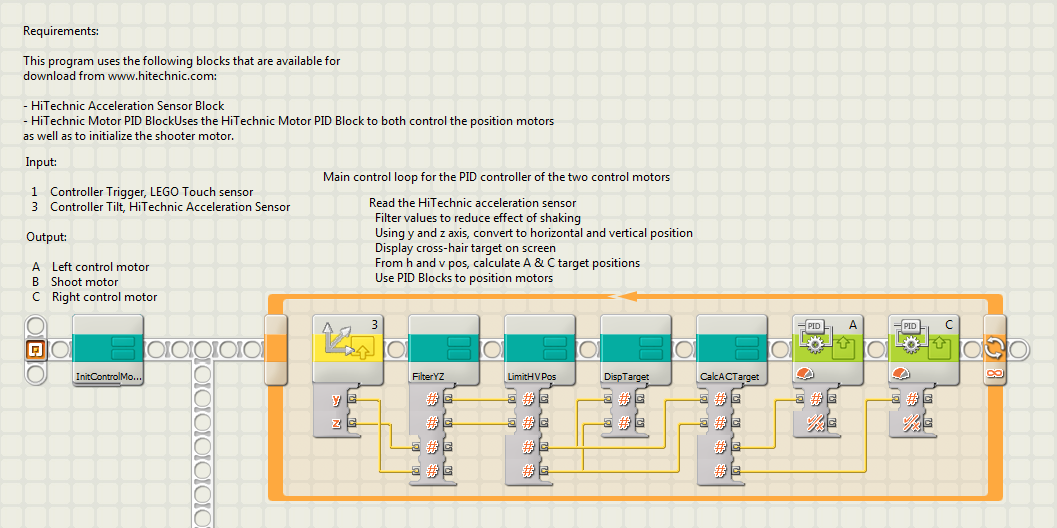
\includegraphics[scale=0.6]{img/SW_main1.png}\\
				Main program (1).
			\end{center}

			\begin{center}
				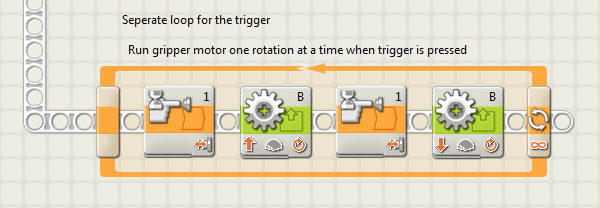
\includegraphics[scale=0.8]{img/SW_main2.png}\\
				Main program (2).
			\end{center}

	\begin{multicols}{2}

			Inside the main structure of the program there are several blocks which are encapsulations of other subprograms to control the robotic arm. These are:\\

			\begin{itemize}
				\item Init Control Motors\\
				
				Set the initial positions of the two motors of the robotic arm. This subblock uses PID block to establish the limits of the motors and in this way controlling the later movements of the operator replicated will not be out of the established ranges.
			\end{itemize}

	\end{multicols}

			\begin{center}
				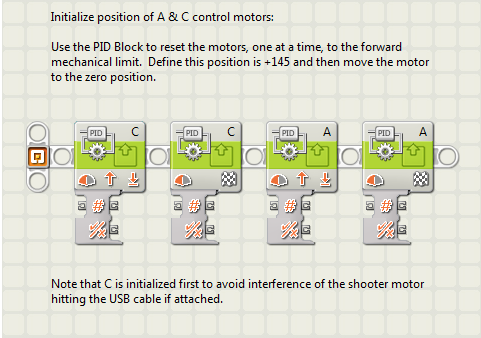
\includegraphics[scale=0.8]{img/SW_InitControlMotors.png}\\
				Init Control Motors.
			\end{center}

	\begin{multicols}{2}

			\begin{itemize}
				\item Filter Y-Z\\
				
				This block performs a low-pass filter to the acceleration values of Y and Z. This is done because it reduces jerkyness caused by the slight shake of the controller. The equation used, as shown in the image, is $vOut(i) = vln(i) * 0.2 + vOut(i - 1) * 0.8$.
			\end{itemize}

	\end{multicols}

			\begin{center}
				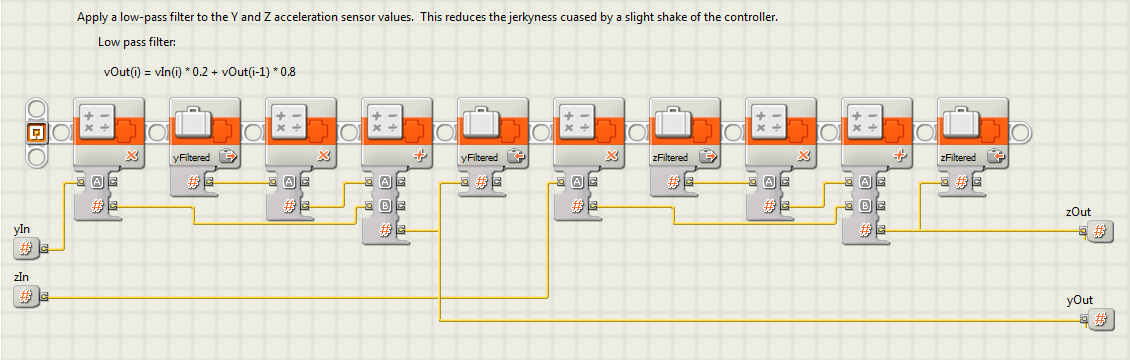
\includegraphics[scale=0.5]{img/SW_FilterYZ.png}\\
				Filter Y-Z.
			\end{center}

			\begin{center}
				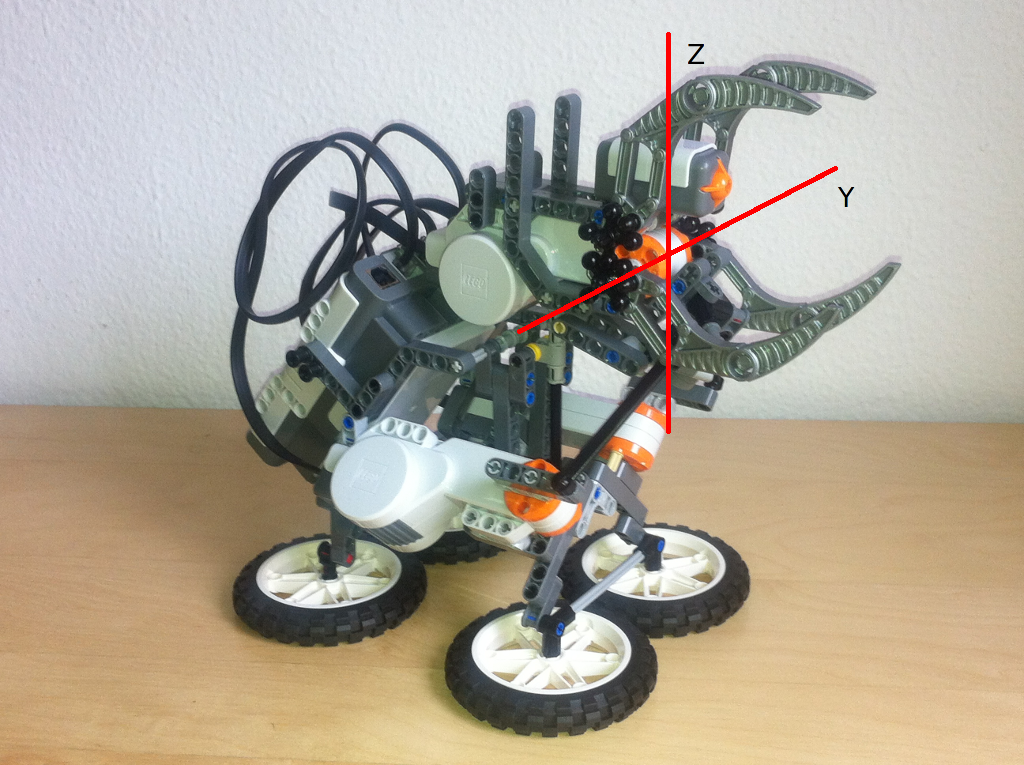
\includegraphics[scale=0.3]{img/robot4.png}\\
				Axes in robotic device.
			\end{center}

	\begin{multicols}{2}

			\begin{itemize}
				\item Limit H/V Position\\
				
				The robotic arm movement will be replicated in two directions, horizontally and vertically. Therefore,  to use the axes Y (horizontal) and Z (vertical). In this case, this block perform the task of limiting the values of the axes so that the movement can be controlled. The ranges of values which are managed, horizontally, from -100 to 100 where the first is the left end and the second the right end which can reach the arm, vertically, from 0 to 100 being the first the lower end and the second the top. These values werw chosen because they are quite intuitive in a traditional coordinate system.
			\end{itemize}

	\end{multicols}

			\begin{center}
				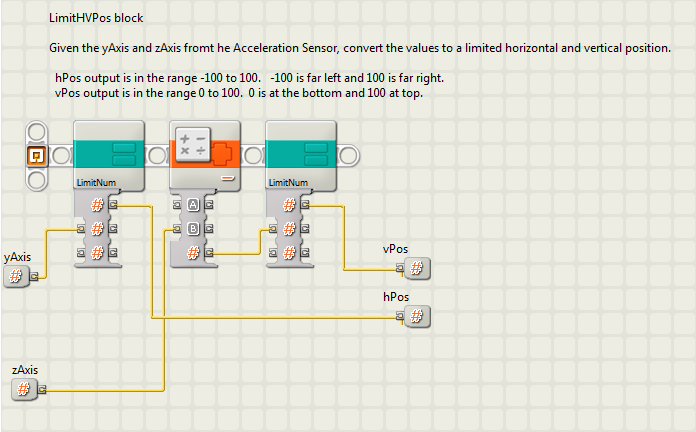
\includegraphics[scale=0.8]{img/SW_LimitHVPos.png}\\
				Limit H/V Position.
			\end{center}

	\begin{multicols}{2}

			\begin{itemize}
				\item Display Target\\
				
				As in any system teleoperated is required to have a feedback that shows how the system is in every moment. In the case of this block which has the function to display on the screen of the NXT brick which the position where is the end of the robotic arm to control at any moment which is within the limits set in which the robot can move . It is a graphical and easy way to make a feedback for the operator who can see the position captured by the system besides to have the option of viewing directly the result in ther own robotic arm.
			\end{itemize}

	\end{multicols}

			\begin{center}
				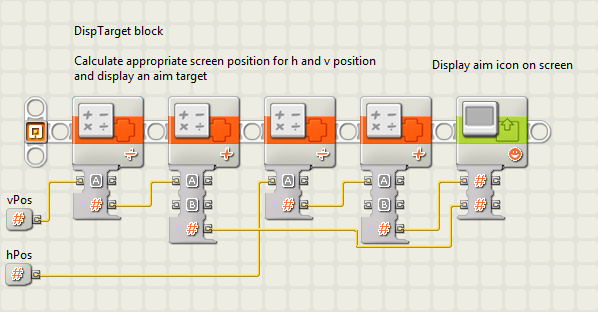
\includegraphics[scale=0.8]{img/SW_DispTarget.png}\\
				Display Target.
			\end{center}

	\begin{multicols}{2}

			\begin{itemize}
				\item Calc AC Target\\
				
				This block calculates the relative positions that will take the robot, these positions will be transformed into movements for each from motors. Once captured the horizontal and vertical positions
				where the sensor is, is performed a conversion of values and calculate the position of the motor, being the position of the first motor the sum of the scaled values h and v, and the other motor the difference between these values.
			\end{itemize}

	\end{multicols}

			\begin{center}
				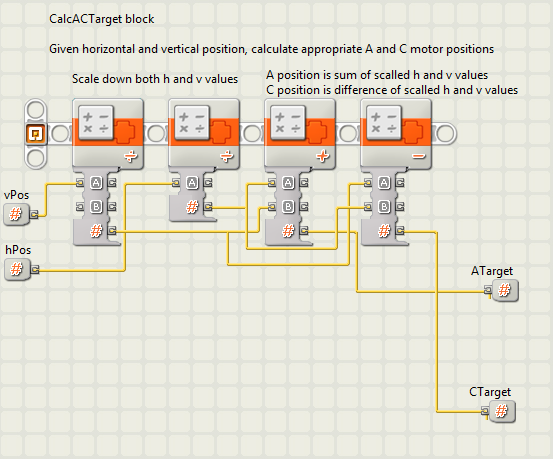
\includegraphics[scale=0.8]{img/SW_CalcACTarget.png}\\
				Calc AC Target.
			\end{center}

	\begin{multicols}{2}

		\ssection{Conclusions}
		
			This section discussed the conclusions obtained from this project.\\

			One of the first conclusions that can be obtained is a teleoperated system is not easy at all, it is necessary that the system has a lot of precision in control and it comes great complexity. However, there are several methods for control, from a PID to intelligent systems using neural networks and evolutive algorithms.\\

			Of course, there are a higher number of future improvements which could be used to improve the system. Since adding artificial vision to recognize where to find the object and calculate the relative position, or add more motors to have more degrees of freedom and the movement of the robotic arm covers a larger space, or include a motorized system for not just a robotic arm, but a moving vehicle with the robotic arm. There are many possible improvements that would make the system increases its complexity and functionality.
		
		\begin{center}
		\section*{References}
		\end{center}
		
			\renewcommand{\labelenumi}{[\theenumi]}
			\begin{enumerate}
				\item Ro-botica. Educative and personal robotic shop. Last visit: Dec-2011.\\
						Link: \href{http://goo.gl/8Yv0H}{http://goo.gl/8Yv0H}
				\item HiTechnic. Last visit: Dec-2011.\\
						Link: \href{http://goo.gl/62Vv6}{http://goo.gl/62Vv6}
				\item G. Sen Gupta, S.C. Mukhopadhyay, C. H. Messom and S. Demidenko. ``Master-Slave Control of a Teleoperated Anthropomorphic Robotic Arm with Gripping Force Sensing". Last visit: Jan-2012.\\
						Link: \href{http://goo.gl/4ZtDe}{http://goo.gl/4ZtDe}
				\item Lesson 3. Teleoperation and Telepresence in Robotic subject.
				\item Lesson 4. Teleoperation and Telepresence in Robotic subject.
				\item Vertut, Jean. Ed. Hermes. ``Teleoperation and robotics. Evolution and development". 1985.
				\item Marc C. Bequet. Ed. Kluwer Academic. ``Teleoperation, numerical simulation and experimental validation". 1992.
			\end{enumerate}

	\end{multicols}

	\vspace{1cm}
	\begin{center}
	
		%LICENCIA
		
\includegraphics[scale=0.8]{img/cc.png}\\
		This work by Raúl Pérula Martínez is under a license \href{http://creativecommons.org/licenses/by-nc-sa/3.0/}{Creative Commons Attribution-NonCommercial-ShareAlike 3.0 Unported}.

	\end{center}
	
\end{document}
